\section{Introduction}
\label{sec:intro}

Reported COVID-19 cases are a staple in tracking the pandemic at varying
geographic resolutions \citep{dong2020interactive, nyt2020corona,
wp2020tracking}. Yet, for every case that is eventually reported to public
health, several infections are likely to have occurred, and likely much earlier. To
see why, it is important to understand \emph{whose} cases are being reported and
what differentiates them from the unreported cases as well as \emph{when} these
case reports happen. \autoref{fig:chain_events_onset_report} shows an
illustration of the path of a symptomatic infection that is eventually
reported to public health. Using this figure, we can discern a number of sources
of bias in the reporting pipeline. For instance, diagnostic testing mainly
targets symptomatic individuals; thus, infected individuals exhibiting little to
no symptoms are omitted \citep{cdc2022estimated}. In addition, testing
practices, availability, and uptake vary temporally and spatially
\citep{pitzer2021impact, ecdc2020strategies, hitchings2021usefulness}. Finally,
cases provide a belated view of the pandemic's progression, because they are
subject to delays due to the viral incubation period, the speed and severity of
symptom onset, laboratory confirmation, test turnaround times, and eventual
submission to public health \citep{pellis2021challenges, wash2020dash}. For
these reasons, reported cases are a lagging indicator of the course of the
pandemic. Furthermore, they do not represent the actual number of new infections
that occur on a given day based on exposure to the pathogen. Since there
was no large-scale surveillance effort in the United States that reliably
tracked symptom onset, let alone infection onset, ascertaining the onset of all
\emph{infections} is challenging.

\begin{figure}[!tb]
\centering
    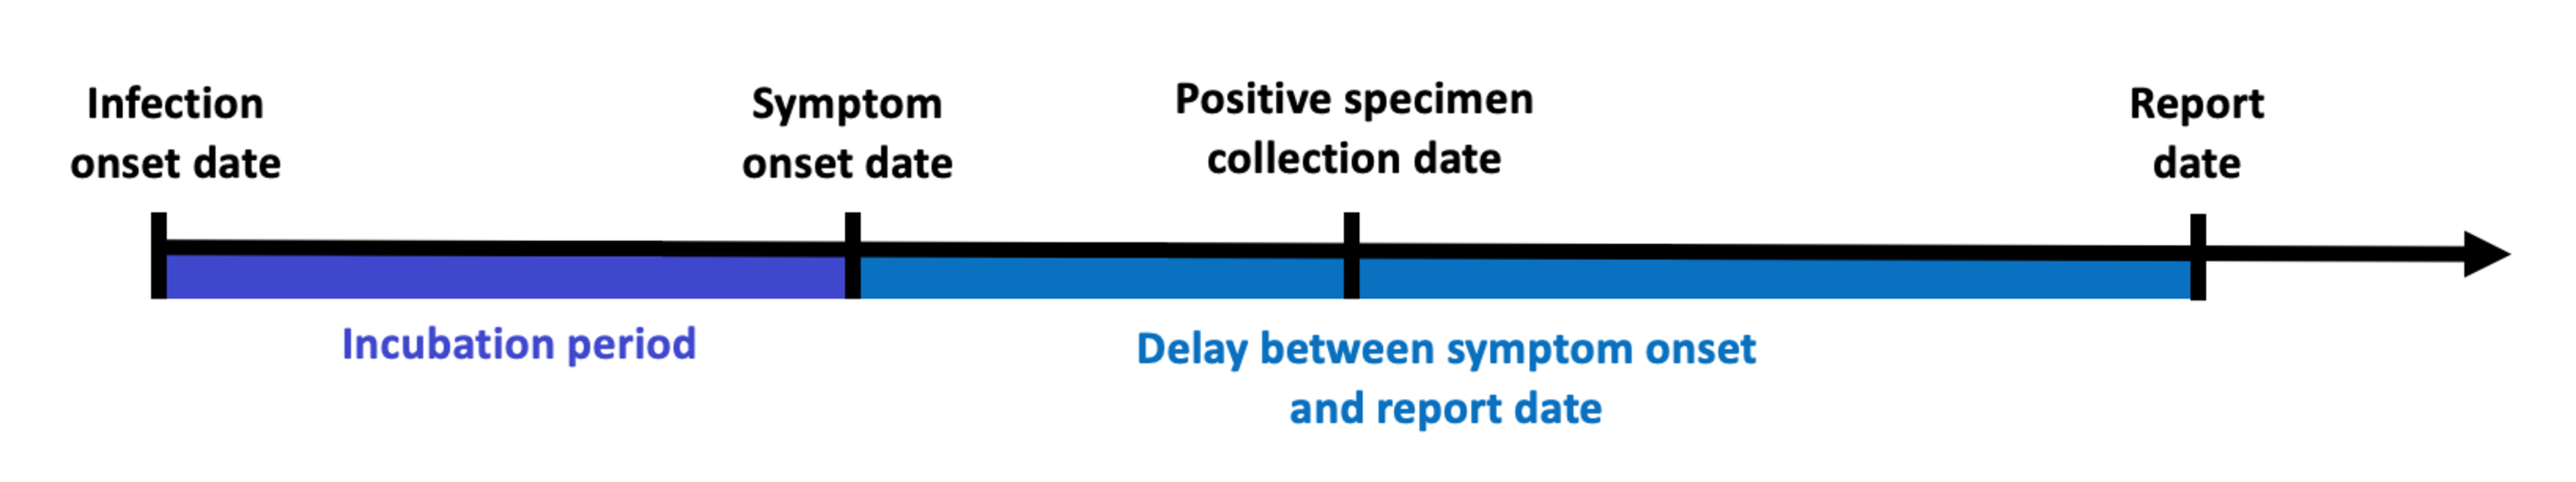
\includegraphics[width=.99\textwidth]{Chain_of_events_onset_report.pdf} 
    \caption{Idealized chain of events from infection onset to case report date 
    for a symptomatic infection that is eventually reported to public health.}
    \label{fig:chain_events_onset_report}
\end{figure}

% Importantly, all of these issues that are present in local health authority
% data are also present in the gold standard for case data from the JHU CSSE
% \citep{dong2020interactive, guidotti2022worldwide} because JHU scrapes case
% data from the local health authority dashboards \citep{jahja2022real}.
% Furthermore, the cases shown on the JHU CSSE Coronavirus Resource Center
% \citep{jhucsse2020covid} are those that have been disseminated to the public
% on a given day. 
% Our approach to estimate latent infections takes case data and estimates the 
% following...

Understanding the course of the pandemic, the effects of interventions and drawing 
insights from this for future pandemics is challenging because the true spatial 
and temporal behaviour of infections is unknown.
While reported cases provide a convenient proxy of the
disease burden in a population, it is incomplete, delayed, and
misrepresents the true size and timing of the pandemic. 
Regardless of these difficulties, it is important to
the public and public health to perform a pandemic post-mortem and try to better
explain its implications---to attempt to capture the true size and impact of the
pandemic as much as we can. Estimates of daily incident infections are one such
way to measure this and can guide understanding of the pandemic burden over
space and time. 

In this work, we provide a data-driven reconstruction of
daily incident infections for each \US state from June 1, 2020 to November 29,
2021. Using state-level line list data, we construct time-varying delay
distributions for the time from symptom onset to positive specimen date and
positive specimen to case report date. We combine these with variant-specific
incubation period distributions to deconvolve daily reported COVID-19 cases back
to their infection onset. Finally, we adjust for the unreported infections 
by using seroprevalence and reinfection data to account for the 
waning of antibody detectability over time. We then
examine some features of our infection estimates and the implications of using
them rather than reported cases in assessing the impact of the pandemic. To this end,
we produce simple time-varying infection-hospitalization ratios (IHRs) for each
state and compare those to similarly derived case-hospitalization ratios (CHRs).
While these analyses provide a glimpse into the utility of our infection
estimates, we believe that there is much more to be explored, and we hope that
our work and publicly-available estimates will prove an
important benchmark for others to undertake retrospective analyses. These estimates
as well as the R and Python code used to produce them can be found at
\href{https://github.com/cmu-delphi/latent-infections/}{https://github.com/cmu-delphi/latent-infections/}.

